\chapter{Lecture}\label{part1:lec3}
\markboth{\thechapter. Lecture}{\thechapter. Lecture}

The\pageoriginale  series $\sum\limits^\infty_{k=0} \mathfrak{z}^k A_k (x)$ that we
had last time is itself rather interesting; the $A_k (x)$ have a queer
shape:
$$
A_k (x) = \frac{x^{k(k-1)/2}}{(1-x)(1-x^2)\cdots (1-x^k)}
$$

Such series are called Euler series. Such expressions in which the
factors in the denominator are increasing in this way have been used
for wide generalisations of hypergeometric series. Euler indeed solved
the problem of computing the coefficients numerically. The coefficient
of $\mathfrak{z}^k x^m$ is obtained by expanding $\frac{1}{(1-x)\cdots
  (1-x^k)}$ as a power series. This is rather trivial if we are in the
field of complex numbers, since we can then have a decomposition into
partial fractions. Euler did find a nice sort of recursion
formula. There is therefore a good deal to be said for a rather
elementary treatment.

We shall, however, proceed to more important discussions the problem
of unrestricted partitions. Consider the infinite product (this is
justifiable modulo $x^N$)
\begin{align*}
  \prod^\infty_{m=1} \frac{1}{1-x^m} & = \prod^\infty_{m=1}
  \sum^\infty_{n=0} x^{mn}\\
  & = \sum^\infty_{n_1=0} x^{n_1} \sum^\infty_{n_2=0} x^{2n_2}\cdot 
  \sum^\infty_{n_j=0} x^{3n_3} \cdots\\
  & = 1+ x+2x^2 + \cdots \\
  & = 1 + \sum^\infty_{n=1} p_n x^n \tag{1}\label{part1:lec3:eq1}
\end{align*}

What\pageoriginale  does $p_n$ signify? $p_n$ appeared in collecting the term
$x^n$. Following Euler's idea of addition of exponents, we have
\begin{equation*}
  n=n_1+ 2n_2+ 3n_3+ 4n_4 + \cdots n_j \geq 0, \tag{2}\label{part1:lec3:eq2}
\end{equation*}
so that $p_n$ is the number of solutions of a \textit{finite}
Diophantine equation (since the right side of (\ref{part1:lec3:eq2}) becomes void after a
finite stage) or the number of ways in which $n$ can be expressed in
this way, or the number of unrestricted partitions. Euler wrote this
as 
\begin{equation*}
  \frac{1}{\prod^\infty_{m=1} (1- x^m)} = \sum^\infty_{n=0} p(n) x^n,
  \tag{3}\label{part1:lec3:eq3} 
\end{equation*}
with the provide that $p(0)=1$.

We want to find as much as possible about $p(n)$. Let us calculate
$p(n)$. Expanding the product,
\begin{align*}
  \prod^\infty_{n=1} (1-x^n) & = (1-x)(1-x^2) (1-x^3)\cdots\\
  & = 1-x-x^2 + x^5+x^7 -x^{12} - x^{15} + + -- \cdots
\end{align*}

(Note Euler's skill and patience; he calculated up to $x^n$ and found
to this surprise that the coefficients were always $0$, $\pm 1$, two
positive terms followed by two negative terms). We want to find the
law of exponents, as every sensible man would. Writing down the first
few coefficients and taking differences, we have 

\medskip
\noindent 
\begin{tabular}{cccccccccccccccccc}
  0 && 1 && 2 && 5 && 7 && 12 && 15 && 22 && 26\\[5pt]
  &$\underline{1}$ && 1 && $\underline{3}$&&2&& $\underline{5}$ && 3&&
  $\underline{7}$ &&4  
\end{tabular}

\medskip 
\noindent 
the sequence of odd numbers interspersed with the sequence of natural
numbers. Euler forecast by induction what the general power would be
as\pageoriginale  follows.

\medskip 
\begin{center}
  \begin{tabular}{cccccccccccccc}
    7&&2&&0&&1&&5&&12&&22&\\[5pt]
    &$-5$&&$-2$&&1&&4&&7&&10&\\[5pt]
    &&3&&3&&3&&3&&3&&&
  \end{tabular}
\end{center}

Write down the coefficients by picking up 0, 1 and every other
alternate term, and continue the row towards the left by putting in
the remaining coefficients. Now we find that the second differences
have the constant value 3. But an arithmetical progression of the
second order can be expressed as a polynomial of the second
degree. The typical coefficient will therefore be given by an
expression of the form
\medskip

    $a \lambda^2 + b\lambda+c$ \qquad  $a(\lambda+1)^2 + b(\lambda+1)+c$
    \qquad $a(\lambda+2)^2 + b(\lambda+2)+c$\\

     \hspace{1.5cm} $a(2 \lambda+1)+b$ \hspace{2cm} $a(2\lambda +3) +
     b$\hspace{4cm}\\  

     \hspace{5cm} 2 a (the constant second difference) 

Hence $2a=3$ or $a=3/2$. Taking $\lambda= 0$ we find that $c=0$ and
$b=-\frac{1}{2}$, so that the general coefficient has the form
$\frac{\lambda (3 \lambda-1)}{2}$. Observing that when $\lambda$ is
changed to $-\lambda$, $\frac{\lambda(3 \lambda-1)}{2}$ becomes
$\frac{\lambda(3 \lambda+1)}{2}$, the coefficient of $x^{\lambda(3
  \lambda-1)/2}$ is $(-)^\lambda$, and hence 
\begin{equation*}
  \prod^\infty_{n=1} (1-x^n) = \prod^\infty_{\lambda=- \infty}
  (-)^\lambda x^{\lambda(3 \lambda-1)/2}, \tag{4}\label{part1:lec3:eq4}  
\end{equation*}
which is Euler's theorem.

This sequence of numbers $\frac{\lambda(3 \lambda-1)}{2}$ played a
particular role in the middle ages. They are called \textit{pentagonal
numbers} and Euler's theorem is called the pentagonal numbers
theorem. We have the so-called triangular numbers:

\medskip 
\begin{center}
  \begin{tabular}{cccccccccc}
    1&&3&&6&&10&&15&\\[5pt]
    &2&&3&&4&&5&&\\[5pt]
    &&1&&1&&1&&
  \end{tabular}
\end{center}
where\pageoriginale  the second differences are all 1; the square-numbers

\medskip 
\begin{center}
  \begin{tabular}{cccccccccc}
    1&&4&&9&&16&&25&\\[5pt]
    &3&&5&&7&&9&&\\[5pt]
    &&2&&2&&2&&
  \end{tabular}
\end{center}
for which the second difference are always 2; and so on.

\begin{figure}[H]
  \centering{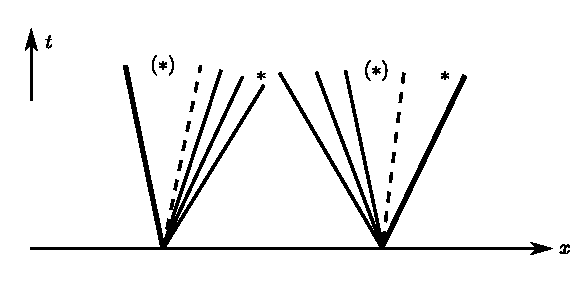
\includegraphics{vol2-figures/fig2.5.eps}}
\end{figure}

The triangular numbers can be represented by dots piled up in the form
of equilateral triangles; the square numbers by successively expanding
squares. The pentagons however do not fit together like this. We start
with one pentagon; notice that the vertices lie perspectively along
rays through the origin. So take two sides as basic and magnify them
and add successive shelves. The second differences now are always 3:

\begin{figure}[H]
\centering{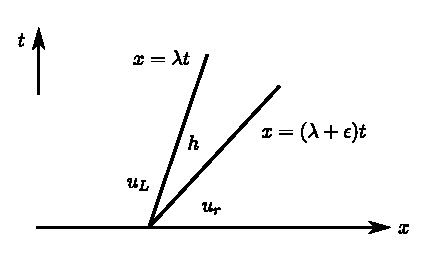
\includegraphics{vol2-figures/fig2.6.eps}}
\end{figure}

In general we can have $r$-gonal numbers where the last difference are
all $r-2$.

We\pageoriginale  go back to equation (\ref{part1:lec3:eq4}):
$$
\prod^\infty_{m=1} (1-x^m)= \sum\limits^\infty_{\lambda=-\infty}
(-)^\lambda x^{\lambda (3\lambda-1)/2} 
$$

It is quite interesting to go into the history of this. It appeared in
Euler's Introduction in Analysin Infinitorum, Caput XVI, de Partitio
numerorum, 1748 (the first book on the differential and integral
calculus). It was actually discovered earlier and was mentioned in a
paper communicated to the St. Petersburgh Academy in 1741, and in
letters to Nicholas Bernoulli (1742) and Goldbach (1743). The proof
that bothered him for nine years was first given in a letter dated 9th
june 1750 to Goldvach, and was printed in 1750.

The identity (\ref{part1:lec3:eq4}) is remarkable; it was the first time in history that
an identity belonging to the $\mathcal{V}$-functions appeared (later
invented and studied systematically by Jocobi). The interesting fact
is that we have a power-series in which the exponents are of the
second degree in the subscripts. The $\mathcal{V}$-functions have a
representation as a series and also as an infinite product.

The proof of identity (\ref{part1:lec3:eq4}) is quite exciting and elementary. By using
distributivity  we break up the product
$$
(1-x)(1-x^2)(1-x^3)(1-x^4)\cdots
$$
in the following way:
\begin{multline*}
  (1-x)(1-x^2)(1-x^3)(1-x^4)\cdots
  = 1-x-(1-x)x^2-(1-x)(1-x^2)x^3-\\
  (1-x)(1-x^2)(1-x^3)(1-x^4)-(1-x)\cdots (1-x^4)x^5- \cdots
\end{multline*}
which may be re-arranged, opening first parenthesis, as
\[
\xymatrix@C=-.01cm{
  \ar@{-}[dr] 1-x-x^2 & -\,(1-x^2)x^3\ar@{-}[dr] & -\,
  (1-x^2)(1-x^3)x^4\ar@{-}[dr] & -\,(1-x^2)(1-x^3)(1-x^4)x^5\ar@{-}[dr]& \\ 
  & + x^3 & + (1-x^2)x^4 & + (1-x^2)(1-x^3)x^5&  }
\]
So\pageoriginale  \quad 
\begin{multline*}
  1-x-x^2+x^5+x^7 (1-x^2)+ x^9 (1-x^2)(1-x^3)+\cdots\\
  \xymatrix@C=-.01cm{= 1-x-x^2+ x^5 + & 2^7 \ar@{-}[dr] & + (1-x^3)x^9
    \ar@{-}[dr] & + (1-x^3) (1-x^4)x^{11}\ar@{-}[dr]& \\
  & & -x^9 & -(1-x^3)x^{11} & &}\\
  1-x-x^2+x^5+x^7 -x^{12}(1-x^3) x^{15} -(1-x^3)(1-x^4)x^{18}-\cdots
\end{multline*}

When this is continued, we get some free terms at the beginning
followed by a typical remainder
$$
(1-x^k)x^m + (1-x^k)(1-x^{k+1})x^{m+k} + (1-x^k)(1-x^{k+1})(1-x^{k+2})
x^{m+2k}, 
$$
which may be rearranged into
\begin{align*}
  x^m & + (1-x^{k+1}) x^{m+k} + (1-x^{k+1}) (1-x^{k+2}) x^{m+2k}-
  x^{m+k} - (1-x^{k+1}) x^{m+2k}\tag{*}\label{part1:lec3:eq*}\\
  & = x^m - x^{m+2k+1} - (1-x^{k+1}) x^{m+3k+2}- (1-x^{k+1})
  (1-x^{k+2})\\
   & \hspace{7.5cm}x^{m+4k+3}- \cdots \tag{**}\label{part1:lec3:eq**}
\end{align*}

We have two free terms with opposite signs at the beginning. In
(\ref{part1:lec3:eq*})
the difference between exponents in successive terms is $k$, while in
(\ref{part1:lec3:eq**}) this increases to $k+1$; this difference is in
both cases the 
exponent of $x$ in the first factor. The remainder after the free
terms begine with $-$, so that the sequence of signs is $+ -- ++ --
\cdots$ This\pageoriginale  process perpetuates itself and the question remains which
powers actually appear. It is sufficient to mark down a scheme for the
exponents which completely characterises the expansion. The scheme is
illustrated by what follows.

\medskip
\noindent 
\tabcolsep=4.8pt
\begin{tabular}{rrrrrrrrrrrrrrrrr}
  0&1&2&3&4&5&6&7&8&9&10&11&12&13&14&15&16\\
  &&&2&3&4&5&6&7&8&9&10&11&12&13&14&15\\
  \cline{4-17}
  &&&5&7&9&11&13&15&17&19&21&23&25&27&29&31\\
  &&&&&3&4&5&6&7&8&9&10&11&12&13&14\\
  \cline{6-17}
  &&&&&12&15&18&21&24&27&30&33&36&39&42&45\\
  &&&&&&&4&5&6&7&8&9&10&11&12&13\\
  \cline{8-17}
  &&&&&&&22&26&30&34&38&42&46&50&54&58\\
  &&&&&&&&&5&6&7&8&9&10&11&12\\
  \cline{10-17}
  &&&&&&&&&35&40&45&50&55&60&65&70\\
  &&&&&&&&&&&6&7&8&9&10&11\\
  \cline{12-17}
  &&&&&&&&&&&51&57&63&69&75&81
\end{tabular}
\medskip

We write down the sequence of natural numbers in a row; the sequence
less the first two members is repeated in a parallel row below leaving
out the first three places at the beginning. Adding up we get
$$
5 \quad 7 \quad 9 \quad 11 \quad \dots ~\dots~\dots\quad, 
$$
below which is placed the original sequence less the first three
members, again translating the whole to the right by two places. We
again add up and repeat the procedure. A typical stage in the
procedure is exhibited below.

\medskip
\begin{center}
  \begin{tabular}{>{$}c<{$}>{$}c<{$}>{$}c<{$}>{$}c<{$}>{$}c<{$}>{$}c<{$}}
    m & m+k & m+2k & m+3k & m+ 4k & m+5k\\
    & k+1 & k+2 & k+3 & k+4 & k+5 \\
    \cline{1-6}
    & m +2k+1 & m+3k+2 & m+4k+3 & m+5k+4 & m+6k+5
  \end{tabular}
\end{center}

The\pageoriginale  free indices then appear successively as 
\begin{alignat*}{4}
  2+3 & = 5 &\qquad \qquad & 3+4+5&= 12\\
  3+4 & = 7 & & 4+5+6& = 15,
\end{alignat*}
and in general:
\begin{align*}
  \lambda + (\lambda+1) + \cdots + (2 \lambda-1) & = \frac{\lambda(3
    \lambda -1)}{2},\\
  (\lambda+1) + (\lambda+2) + \cdots + 2 \lambda & = \frac{\lambda(3
    \lambda+1)}{2}, 
\end{align*}
which are the only exponents appearing. We thus have
$$
\prod^\infty_{n=1} (1-x^n) = \sum^\infty_{\lambda=-\infty} (-)^\lambda
x^{\lambda(3 \lambda -1)/2}
$$
